\documentclass[11pt]{article}

\usepackage[utf8]{inputenc}
\usepackage[T1]{fontenc}
\usepackage[margin=1in]{geometry}
\usepackage{hyperref}
\usepackage{natbib}
\usepackage{enumitem}
\usepackage{parskip}
\usepackage{longtable}
\usepackage{array}
\usepackage{booktabs}
\usepackage{tikz}
\usetikzlibrary{shapes.geometric, arrows.meta, positioning}

\hypersetup{
    colorlinks=true,
    linkcolor=blue,
    urlcolor=blue,
    citecolor=blue,
    pdftitle={Test-Taker Experiences of Standardized Testing: A Scoping Review},
    pdfauthor={Sergio Araneda}
}

\title{Test-Taker Experiences of Standardized Testing:\\ A Scoping Literature Review\\[6pt]
\large\textit{An automatically machine-generated draft, prepared by the TTX Automatic Literature Reviewer pipeline --\\ to be treated as an experiment in automated literature synthesis, not an official literature review}}
\author{Sergio Araneda \\ Caveon \\ Correspondence: \texttt{sondaxius@gmail.com}}
\date{\today}

\begin{document}

\maketitle

\begin{abstract}
\noindent This review synthesizes 56 open-access records on the lived experience of taking standardized and high-stakes tests, drawn from a corpus assembled by an automated, continuously-running literature-scanning pipeline across three source categories reported separately so their conclusions can be compared rather than blended: 30 preprints and repository items, 25 peer-reviewed journal articles, and 1 news article. The corpus spans educational, language-testing, and personnel-selection contexts and covers recurring dimensions of test-taker experience: the psychological and physiological toll of high-stakes testing (anxiety, stress, measurable biomarker responses); perceptions of fairness and reactions to testing outcomes, procedures, and teachers' own accounts of administering high-stakes tests; how the mode of test delivery -- paper, computer, video, or AI-mediated -- shapes test-takers' comfort and trust; and the surveillance and privacy tensions introduced by remote proctoring. Every paper is mapped onto the three-dimensional conceptual framework for Test-Taker eXperience (TTX) proposed by \citet{araneda2025ttxmodel} (temporal stage, type of interaction, level of sense-making), and the concrete invalidity hypothesis each paper's findings suggest is listed against the five-type invalidity taxonomy from \citet{araneda2023dissertation}. A cross-source finding illustrates why separating conclusions by source matters: a claim in an earlier version of this review that no genuinely relevant Spanish-language material existed in the accessible literature turned out to be true only of the preprint corpus -- five Spanish-language peer-reviewed papers survived an identical screening process once a peer-reviewed source was added, while French-language coverage remains thin across every source tried. A PRISMA-style flow diagram, a full methodology section, and an explicit discussion of what this review would still need for formal PRISMA compliance make the review's evidentiary basis auditable and reproducible.
\end{abstract}

\section{Introduction}

Standardized tests mediate some of the most consequential decisions in a person's academic and professional life: university admission, professional licensure, immigration eligibility, and school accountability all lean on the assumption that a test score is a fair, stable, and interpretable signal. Historically, the research literature on standardized testing has been dominated by the psychometric perspective -- reliability, validity, item response theory -- with comparatively less attention paid to the perspective of the person sitting the test. Over the last decade, however, a distinct and growing body of work has begun to treat the \emph{test-taker's experience} as a legitimate object of study in its own right: how test-takers feel before, during, and after a test; how they interpret and react to the fairness of the process; how new modes of delivery (computer-based, video-mediated, AI-proctored) change that experience; and how teachers and institutions perceive the effects of high-stakes testing on the people subjected to it.

This review asks: \emph{what does the currently accessible open-access and preprint literature reveal about how test-takers experience standardized and high-stakes testing, across psychological, procedural, technological, and institutional dimensions?} It is deliberately scoped to what an automated, multilingual, daily-running literature scanner can currently retrieve and verify as relevant -- not a claim to exhaustive coverage of the field. Section~\ref{sec:methodology} documents exactly how the underlying corpus was assembled, filtered, and screened, so that the scope and limits of the synthesis that follows are transparent.

\section{Conceptual Framework: The TTX Model}
\label{sec:ttxmodel}

To move beyond an unstructured thematic synthesis, this review adopts a published conceptual framework for test-taker experience rather than inventing an ad hoc one. \citet{araneda2025ttxmodel} propose a model for \emph{Test-Taker eXperience} (TTX) -- a term originating with researchers at Duolingo \citep{burstein2021ttxorigin} -- built from three orthogonal dimensions, and \citet{araneda2023dissertation} extends this model into a taxonomy of \emph{invalidity hypotheses} that test-taker experience evidence can surface. Both are used here to organize the corpus, not merely to summarize it.

\subsection{Three Dimensions of Test-Taker Experience}

Drawing on Dewey's \citeyearpar{dewey1938} principles of continuity, interaction, and sense-making, and on Forlizzi and Battarbee's \citeyearpar{forlizzi2004} interaction-centered model of user experience, \citet{araneda2025ttxmodel} define test-taker experience along three dimensions:

\begin{description}[leftmargin=3.6cm, style=nextline]
    \item[Temporal stage] \emph{When}, relative to the test itself, the experience occurs: \textbf{ante-experience} (well before an examinee starts preparing), \textbf{pre-experience} (preparing, once taking the test is certain), \textbf{zero-experience} (during the test), \textbf{inter-post experience} (between taking the test and receiving results), \textbf{post experience} (immediately after receiving results), and \textbf{long-term experience} (well after results are received).
    \item[Type of interaction] \emph{What kind} of encounter between examinee and test is involved: \textbf{fluent} (automatic, pre-conscious, e.g. navigating a familiar interface), \textbf{cognitive} (effortful mental processing), \textbf{emotional} (affect -- anxiety, boredom, fun), \textbf{expressive} (self-expression in reaction to the test), and \textbf{physical} (bodily interactions and needs, including physiological stress responses).
    \item[Level of sense-making] \emph{How processed} the experience is when reported: \textbf{free-stream} (raw, barely-processed stream of self-talk), \textbf{immediate} (an initial, incomplete integration of something that just happened), \textbf{integrative} (a complete narrative with a beginning and end, constructed alone), \textbf{co-integrative} (the same, but co-constructed with peers, teachers, or other stakeholders), and \textbf{dialogical} (co-constructed specifically with the test designer, e.g. through public comments to a testing agency).
\end{description}

These dimensions are designed to be crossed: a given piece of evidence about test-taker experience -- a tweet, a survey response, an interview transcript -- can in principle be located at a specific temporal stage, interaction type, and sense-making level simultaneously.

\subsection{Five Types of Invalidity Hypotheses}

\citet{araneda2023dissertation} connects test-taker experience evidence directly to test validation by proposing that a validity argument answer four questions -- the \textbf{P.A.A.P. minimum}: is the argument \emph{Partial} and situated (acknowledging whose perspective it represents)? Is the test \emph{Appropriate} (ethical to use)? Is it \emph{Adequate} (scientifically sound for its construct)? Is it \emph{Preferable} to other adequate, appropriate alternatives? Correspondingly, five types of invalidity can be surfaced from test-taker experience evidence:

\begin{description}[leftmargin=3.6cm, style=nextline]
    \item[Value rejection] (Appropriateness) An ethical objection to the test itself.
    \item[Construct under-representation] (Adequacy) The test, or part of it, fails to capture an aspect of the construct it was meant to measure.
    \item[Construct-irrelevant interaction] (Adequacy) An interaction between examinee and test occurs that is spurious to the construct being measured (the classic example is test anxiety inflating or deflating a score independent of the ability being assessed).
    \item[Purpose misfit] (Adequacy) The test fails at its purpose as a measurement device -- e.g., its reliability or error structure does not fit the needs of the context in which it is used.
    \item[Failed test expectation] (Preferability) A side expectation not directly tied to the test's core purpose -- a societal goal, an experiential requirement -- goes unmet.
\end{description}

Unlike a conventional threats-to-validity checklist, this taxonomy is explicitly meant to be populated \emph{from} test-taker experience evidence: a researcher studies examinees' (and other stakeholders') experiences, generates invalidity hypotheses grounded in what was observed or reported, and then investigates each hypothesis with further evidence. Sections~\ref{sec:mapping} and~\ref{sec:invalidity} apply both parts of this framework -- the three experience dimensions and the five invalidity types -- to the 30-paper corpus described in Section~\ref{sec:methodology}.

\section{Methodology}
\label{sec:methodology}

\subsection{Automated Search Pipeline}

The corpus underlying this review is produced by an automated pipeline (the \emph{TTX Automatic Literature Reviewer}) that runs daily and queries four free, key-free sources at the time of writing, one per source category described in the Findings sections below: \textbf{SHARE} (\texttt{share.osf.io}), an aggregator that indexes OSF's own preprint servers (PsyArXiv, EdArXiv, SocArXiv) alongside hundreds of other open repositories worldwide, and \textbf{arXiv}, together the ``preprints and repositories'' category (Section~\ref{sec:findings-preprints}); \textbf{OpenAlex}, restricted to peer-reviewed journal articles, the ``peer-reviewed journal literature'' category (Section~\ref{sec:findings-openalex}); and the \textbf{GDELT DOC 2.0 API}, a global news index, the ``news and magazine coverage'' category (Section~\ref{sec:findings-news}). Support for a fifth source, \textbf{CORE.ac.uk} -- a large aggregator with substantially stronger non-English open-access coverage -- has been implemented but is not yet enabled pending an API key.

For each of three target languages (English, Spanish, French), every source is queried for records that contain at least one term from a curated \emph{topic} set (e.g., \textit{standardized test}, \textit{high-stakes testing}, \textit{test taker}) \textbf{and} at least one term from a curated \emph{experience} set (e.g., \textit{test anxiety}, \textit{perceptions}, \textit{wellbeing}, \textit{stress}, \textit{fairness}). This two-group query structure is intended to bias retrieval toward records that are about both standardized testing \emph{and} the subjective experience of it, rather than standardized testing in general.

Following the adoption of the TTX model (Section~\ref{sec:ttxmodel}), the experience-term set and the client-side relevance gate (Section~\ref{sec:relevance}) were extended with the model's own vocabulary -- \textit{assessment experience}, \textit{construct-irrelevant}, and \textit{invalidity hypothesis} -- so that future runs of the pipeline explicitly recognize literature that engages with this framework or its terminology, rather than relying only on the generic testing/experience terms used to build the corpus analyzed in this version of the review.

\subsection{Relevance Filtering}
\label{sec:relevance}

Different search backends match and rank free text inconsistently -- some effectively required all query terms to be present, others scored by partial overlap, which in early testing let single generic words (e.g., a Spanish-language paper matching only on \textit{estudiantil}, ``student-related'') pull in clearly unrelated records. To compensate, every candidate record from every source -- including snowballed candidates, see below -- is passed through a second, client-side relevance gate: a record is retained only if its title and abstract, normalized for case and accent, contain at least one phrase from a curated relevance-keyword list spanning all three target languages.

\subsection{Snowballing}
\label{sec:snowball_persistent}

Newly retained records are used as seeds for citation snowballing via the Semantic Scholar Graph API: each seed's \emph{references} (backward snowball), the papers that \emph{cite} it (forward snowball), and Semantic Scholar's \emph{recommendations} (its equivalent of a ``related articles'' panel) are retrieved and passed through the same relevance gate before being added to the corpus. This substitutes for Google Scholar's related-work features, which have no public API and cannot be scraped without violating Google's terms of service.

In addition to seeds found by that day's keyword search, the pipeline now also snowballs every run from a short list of \emph{persistent seeds} -- foundational papers specified directly in configuration, independent of whether they were matched by any query. \citet{araneda2023dissertation} is configured as the first such seed, so that papers which cite or build on the Experiential Approach to test validation are picked up as forward citations even on days the keyword search finds nothing new. When a seed's DOI is not indexed by Semantic Scholar under that identifier -- common for institutional-repository DOIs such as this dissertation's, minted by a university library rather than a journal publisher -- the pipeline falls back to a title search before giving up on that seed for the run.

\subsection{Corpus at Time of Writing}

As of the final run reported in this review (2026-08-13), the pipeline identified 158 raw candidate records across all four sources and languages (Figure~\ref{fig:prisma}), of which 106 passed the automated relevance gate: 24 from arXiv, 27 from SHARE, 54 from OpenAlex, and 1 from GDELT.

\subsection{Manual Screening for This Review}
\label{sec:screening}

The automated keyword gate is a precision heuristic, not a substitute for judgment, and on every source tested it let through records that share vocabulary with the topic but are not substantively about test-taker experience. From SHARE: papers on COVID-19 medical testing, robotics disturbance-rejection benchmarking, general algorithmic-fairness theory that uses ``standardized test scores'' only as an illustrative feature, and, notably, one advertisement for a commercial exam-cheating service that had been indexed by the aggregator as though it were a scholarly record. From OpenAlex: a general motivation-psychology handbook, a standardized behavioral test for aggression in laboratory rats, and studies on livestock farming, portfolio volatility, and childhood asthma epidemiology that matched only on generic term overlap (Section~\ref{sec:findings-openalex}). For this review, all 106 automatically retained records were manually screened against the review question, separately by source category so that each category's screening decisions and yield could be reported on their own terms (Sections~\ref{sec:findings-preprints}--\ref{sec:findings-news}); near-duplicate entries (the same record surfaced independently by more than one query) were also collapsed. This manual pass retained \textbf{30 preprint/repository records}, \textbf{25 peer-reviewed journal records}, and \textbf{1 news record} -- 56 records in total, 55 of them synthesized thematically (Sections~\ref{sec:findings-preprints}--\ref{sec:findings-openalex}) and the single news record discussed individually rather than thematically, for the reasons explained in Section~\ref{sec:findings-news}.

An earlier version of this review, built from the preprint/repository corpus alone, reported that no genuinely relevant Spanish- or French-language material existed in the accessible evidence base: all five Spanish-language SHARE records screened out at that stage concerned evaluation research unrelated to test-taker experience (an early-childhood program impact evaluation, a study of armed-conflict ceasefire effects on standardized test scores as an \emph{outcome} measure, an athletics intervention, and similar), matching the automated gate only through generic evaluation-research vocabulary (e.g., \textit{bienestar}, ``wellbeing''; \textit{estandarizada}, ``standardized''). Adding OpenAlex overturned half of that finding: five Spanish-language peer-reviewed papers survived an identical screening process (Section~\ref{sec:findings-openalex}). We now treat the earlier finding as a property of \emph{which sources had been searched} at that point, not of the literature itself -- see the fuller discussion in Section~\ref{sec:crosssource}. The French-language finding has not been overturned by any source added so far and remains open, discussed further in Section~\ref{sec:limitations}.

\subsection{Bibliographic Enrichment}

The pipeline's own metadata store records title, authors, a publication date, an abstract where available, and a DOI or URL, but not a journal or venue name. For this review, venue, volume, issue, and page information were retrieved separately via the Crossref and DataCite public APIs for the subset of records with a resolvable DOI, and cross-checked against the pipeline's recorded publication year (this caught at least one indexing error, discussed in Section~\ref{sec:limitations}).

\subsection{Flow Diagram}
\label{sec:prisma}

This is a scoping synthesis, not a formal systematic review (Section~\ref{sec:limitations} discusses what full PRISMA 2020 compliance would additionally require), but Figure~\ref{fig:prisma} adapts the PRISMA flow-diagram convention to report the identification, screening, eligibility, and inclusion counts for this review's final run with the same transparency a systematic review's diagram would provide.

\begin{figure}[htbp]
\centering
\resizebox{\textwidth}{!}{%
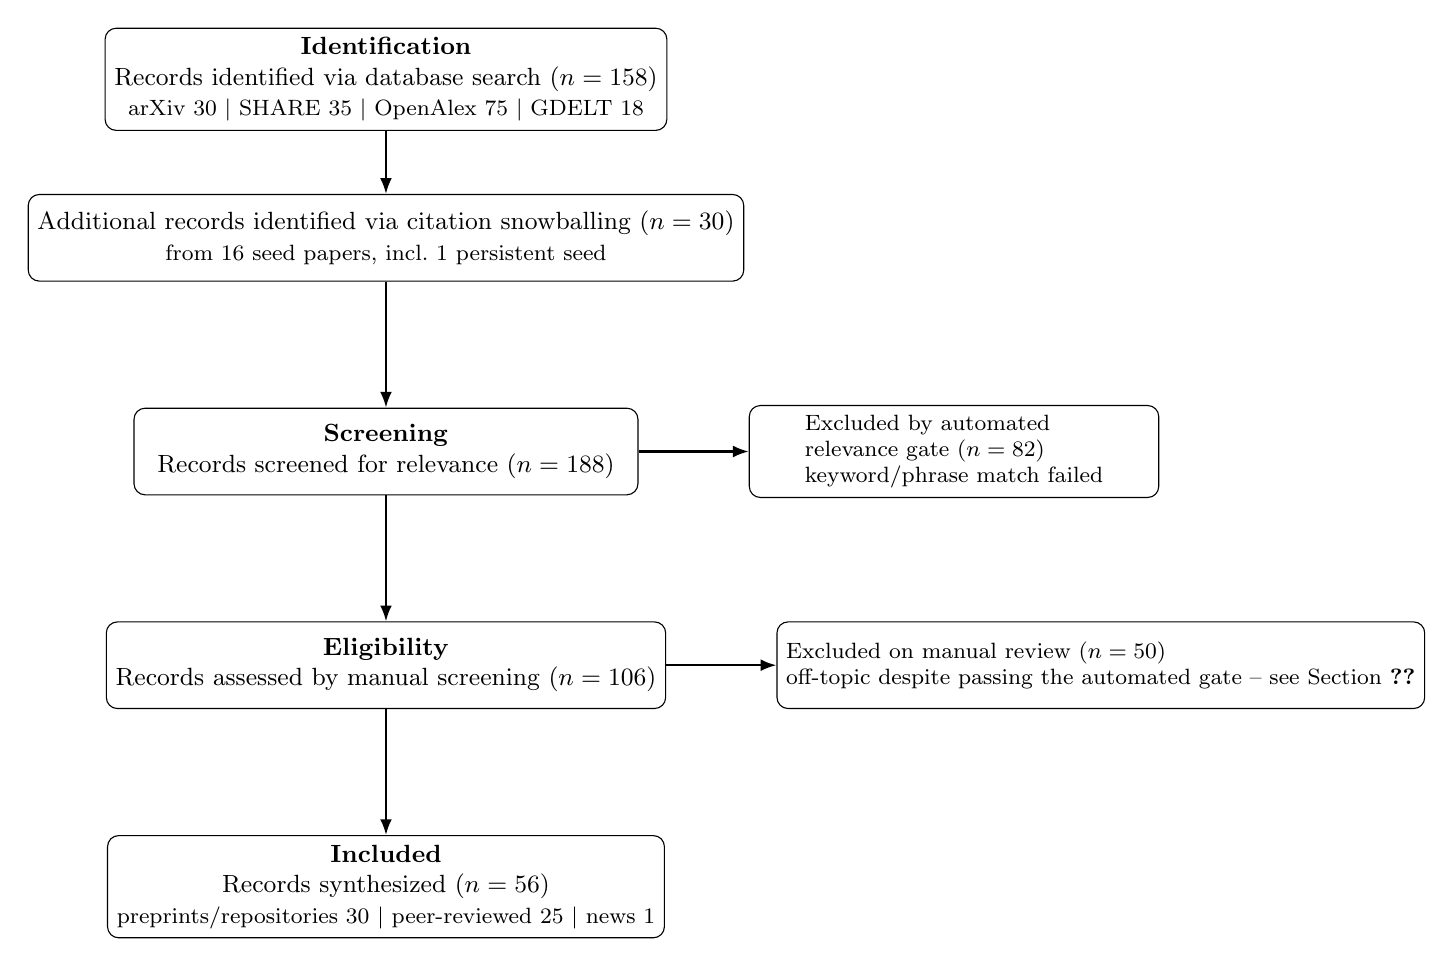
\begin{tikzpicture}[
    node distance=8mm and 14mm,
    box/.style={rectangle, draw, rounded corners, align=center, minimum width=6.4cm, minimum height=1.1cm, font=\small},
    exbox/.style={rectangle, draw, rounded corners, align=left, minimum width=5.2cm, minimum height=1.1cm, font=\footnotesize},
    arr/.style={-{Latex[length=2mm]}, thick}
]

\node[box] (ident) {\textbf{Identification}\\Records identified via database search ($n=158$)\\{\footnotesize arXiv 30 \textbar\ SHARE 35 \textbar\ OpenAlex 75 \textbar\ GDELT 18}};
\node[box, below=of ident] (snow) {Additional records identified via citation snowballing ($n=30$)\\{\footnotesize from 16 seed papers, incl.\ 1 persistent seed}};

\node[box, below=16mm of snow] (screen) {\textbf{Screening}\\Records screened for relevance ($n=188$)};
\node[exbox, right=of screen] (exscreen) {Excluded by automated\\relevance gate ($n=82$)\\{\footnotesize keyword/phrase match failed}};

\node[box, below=16mm of screen] (elig) {\textbf{Eligibility}\\Records assessed by manual screening ($n=106$)};
\node[exbox, right=of elig] (exelig) {Excluded on manual review ($n=50$)\\{\footnotesize off-topic despite passing the automated gate -- see Section~\ref{sec:screening}}};

\node[box, below=16mm of elig] (incl) {\textbf{Included}\\Records synthesized ($n=56$)\\{\footnotesize preprints/repositories 30 \textbar\ peer-reviewed 25 \textbar\ news 1}};

\draw[arr] (ident) -- (snow);
\draw[arr] (snow) -- (screen);
\draw[arr] (screen) -- (elig);
\draw[arr] (elig) -- (incl);
\draw[arr] (screen) -- (exscreen);
\draw[arr] (elig) -- (exelig);

\end{tikzpicture}%
}
\caption{PRISMA-style flow diagram for this review's final run (2026-08-13). ``Screening'' here is the automated keyword relevance gate (Section~\ref{sec:relevance}); ``Eligibility'' is the manual screen described in Section~\ref{sec:screening} and, per source category, in Sections~\ref{sec:findings-preprints}--\ref{sec:findings-news}. No duplicate records were removed at the identification stage in this run.}
\label{fig:prisma}
\end{figure}

\section{Findings from Preprints and Repositories}
\label{sec:findings-preprints}

This section covers the corpus drawn from SHARE and arXiv, plus their citation-snowballed descendants (Section~\ref{sec:snowball_persistent}) -- i.e. preprints and open-repository items, the ``grey literature'' side of the review. Sections~\ref{sec:findings-openalex} and~\ref{sec:findings-news} cover the peer-reviewed and news/magazine corpora separately, so that conclusions can be compared across source categories rather than blended into one undifferentiated pool (see the cross-source comparison in Section~\ref{sec:discussion}).

\subsection{Psychological and Emotional Dimensions of Test-Taking}

The most consistent theme across the corpus is that high-stakes testing carries a measurable psychological cost, and that this cost is treated by researchers as a legitimate target for intervention rather than an unavoidable by-product of assessment. \citet{george2024examstress} frames exam-related student mental health strain as a global, epidemic-scale phenomenon, situating exam-period stress within broader adolescent suicide statistics and arguing for its recognition as a public-health concern rather than a purely educational one. \citet{tseng2024taiwanese} contribute a longitudinal study of high-stakes test anxiety among Taiwanese adolescents, extending this line of work to an East Asian context in which standardized examinations play an outsized role in secondary and tertiary admissions. \citet{wallace2010motivation} likewise examine the relationship between high-stakes testing, motivation, anxiety, and engagement specifically in children, though the source record for this study lacks a machine-readable abstract, so its findings are not characterized further here.

Two studies in the corpus move from documenting test anxiety to actively mitigating it. \citet{amsberry2018sound} report a four-week within-subjects study in which exposure to preferred music during testing improved performance by as much as 22\% relative to silent or non-preferred soundscapes, suggesting that manipulating the testing \emph{environment} -- rather than only the test-taker's coping strategies -- can meaningfully change the experience of high-stakes testing. \citet{watson2026cat} address a more procedural source of anxiety: in computerized adaptive testing (CAT), abrupt jumps in item difficulty between consecutive questions can themselves trigger anxiety and frustration, and the authors propose and compare four algorithmic methods for smoothing difficulty progression specifically to improve test-taker experience. \citet{eleje2023cbtppt} compare computer-based and paper-and-pencil test administration among Nigerian secondary school students, examining both academic achievement and test anxiety as outcomes of delivery mode.

\subsection{Perceptions of Fairness and Reactions to Outcomes}

A second cluster of studies treats fairness not as a statistical property of a test but as something test-takers actively \emph{perceive} and \emph{react to}. \citet{feeney2022rejection} examine how the framing of post-test feedback given to rejected job applicants -- absolute scores versus scores framed relative to other candidates -- shapes applicants' fairness perceptions and their behavioral intentions toward the hiring organization. \citet{stierwalt2000explanations}, in an earlier but closely related study, show that organizational explanations offered for the use of a selection test interact with outcome favorability and test-takers' self-efficacy to jointly shape their perceptions of the test. \citet{zhou2024genderforced} examine gender differences in test-taker reactions to, and fairness perceptions of, multidimensional forced-choice personality measures, a test format increasingly used in personnel selection specifically because it resists faking.

Other work in this cluster addresses fairness at the level of test \emph{content} rather than test \emph{outcomes}. \citet{grand2013sensitivity} study the effectiveness of ``sensitivity review'' practices -- expert review intended to catch test items that could unfairly disadvantage or offend particular groups before they reach test-takers -- and how such problematic content, when missed, affects testing outcomes. \citet{suk2026unfairness} formalize test unfairness for non-manipulable group characteristics (e.g., gender, race, English-language-learner status) through the lens of differential item functioning (DIF), addressing the long-standing methodological question of what it even means to speak of a ``causal effect'' of group membership on item performance. With the rise of AI-assisted test-content generation, \citet{stowe2024fairness} extend this content-fairness concern to automatically generated items for a large-scale English proficiency test, flagging generated content that could disadvantage or distract a subset of test-takers even when it displays none of the more commonly studied forms of model bias. \citet{burstein2024responsible} report a case study of Responsible AI practices at the Duolingo English Test, explicitly framing ``test equity'' -- fairness to all test-takers -- alongside test quality as a governing design principle for AI-powered assessment.

\subsection{Mode of Delivery: Paper, Computer, Video, and AI-Mediated Testing}

A substantial share of the corpus compares how test-takers experience different delivery modes for the same underlying construct. \citet{dang2024vstep} compare computer-delivered and face-to-face administrations of two English speaking-proficiency tests within the Vietnamese Standardized Test of English Proficiency (VSTEP), explicitly incorporating test-takers' own reported experiences alongside score comparability across 75 and 82 test-takers respectively. \citet{nakatsuhara2021videoconferencing} compare video-conferencing and face-to-face administrations of the IELTS Speaking Test with 99 test-takers and 10 trained examiners, finding via Many-Facet Rasch Model analysis that delivery mode did not produce a meaningful difference in test-taker scores. \citet{quaid2021fluency} instead focus on a qualitative dimension largely neglected by score-comparability studies: how test-taker \emph{fluency} -- both spoken output and underlying processing fluency -- is expressed differently in simulated (computer-based) versus face-to-face oral proficiency interviews. \citet{amengual2017views} directly solicit test-takers' own views via an open questionnaire administered to 80 APTIS speaking-test takers, examining the perceived advantages and disadvantages of computer-based relative to face-to-face oral assessment. \citet{nguyen2026examiners} complement this test-taker-facing literature with the examiner's perspective on computer-assisted language testing (CALT), situating growing test-taker familiarity with digital platforms such as IELTS, APTIS, and Duolingo within the broader shift toward digital testing environments.

The newest delivery-mode question in the corpus concerns artificial intelligence. \citet{zhang2023testtakers} report what the authors describe as the first empirical study of test-taker perceptions of AI integration into language testing, based on interviews and surveys with English test-takers: participants perceived AI as potentially enhancing fairness, consistency, and availability, while simultaneously expressing mistrust regarding the reliability and interactivity of AI-mediated testing -- a genuinely mixed reaction that echoes the fairness-versus-trust tension found elsewhere in the corpus.

\subsection{Surveillance, Privacy, and Integrity in Remote Testing}

The shift toward remote and online testing, accelerated by the Covid-19 pandemic, has introduced a distinct experiential concern: being watched. \citet{balash2021examiners} survey students' privacy and security perceptions of online proctoring services, combining an analysis of user reviews of proctoring browser extensions with an online survey (n=102). They find that participants are uneasy about both the volume and the personal nature of information shared with proctoring companies, but many also recognize a trade-off between pandemic-era safety and the invasiveness of proctoring, and that institutional power dynamics and students' trust in their institutions appear to dissuade open opposition to remote proctoring. \citet{mukherjee2024proctoring} probe a possible mitigation: whether selectively obfuscating parts of a proctoring video feed (a test-taker's face, body, or background) can preserve effective cheating detection while improving perceived privacy and fairness. Combining expert interviews (N=9) with a large vignette experiment (N=259 potential test-takers), they find that advanced obfuscation methods (e.g., silhouetting, avatar replacement) improved perceived privacy and fairness relative to conventional blurring, but at some cost to perceived sufficiency of cheating detection -- and that in practice, non-expert participants still preferred the simpler, more familiar blurring method for material they were willing to share, revealing a gap between technically superior privacy protection and what test-takers are actually comfortable adopting.

\subsection{Teacher and Institutional Perspectives on the Student Testing Experience}
\label{sec:teacherperspectives}

Several studies approach test-taker experience indirectly, through the eyes of teachers and other institutional actors rather than test-takers themselves -- a complementary lens, since teachers are often positioned to observe patterns of student stress and disengagement across many individual test-takers. \citet{steuart2024ruralteachers} study rural U.S. teachers' perceptions of how high-stakes testing affects high school students, addressing a rural-versus-urban gap noted in the broader literature, which the author observes has focused disproportionately on urban and diverse school systems. \citet{weick2024instruction} and \citet{reese2004teachersperceptions} both examine teacher perceptions of how high-stakes testing shapes instructional practice, the latter specifically in relation to school leadership. \citet{mccauley2021irish} extend this institutional-perspective literature outside the United States, examining ``key actor'' perspectives -- a category that includes but is not limited to teachers -- on standardised assessment in the Irish primary school context, a system in which the stakes attached to test results are explicitly lower than in more high-stakes national contexts.

\subsection{Systemic and Policy-Level Consequences}

Two studies situate individual test-taker experience within larger systemic or policy dynamics. \citet{zhangw2024naplan} evaluate Australia's National Assessment Program for Literacy and Numeracy (NAPLAN) reform, linking its high-stakes, standardized character to exacerbated student anxiety and stress and to specific inequity for students with a language background other than English (LBOTE), and recommend policy responses including a transition to online testing and increased investment in assessment literacy. \citet{ladant2023saliency} provide causal evidence, using a natural experiment among Italian primary school students, that a \emph{visible} class rank derived from teachers' exam grades has a substantial effect on students' self-perceptions, which in turn affects their subsequent academic performance -- independent of an ``invisible'' rank computed from unreported standardized test scores. This is a useful complication for the broader review: it suggests that test-taker experience is shaped not only by the test itself, but by how test-derived information is socially packaged and disclosed.

\subsection{Test-Taker Response Behavior and Self-Presentation}

A smaller cluster of studies examines how test-takers actively shape their own responses under high-stakes conditions. \citet{kleinbub2026socialdesirability} model how differing perceptions of social desirability among test-takers introduce bias into self-report and forced-choice personnel-selection measures via faking behavior, work that directly extends the Multidimensional Nominal Response Model used to detect such faking. \citet{lee2025forcedchoice} situate this concern within a broader 80-year methodological history, providing a systematic review of forced-choice measurement -- including faking resistance -- that offers useful context for the more specific studies elsewhere in this corpus.

\subsection{A Registered Effort at Synthesis}

One record in the corpus is itself a direct attempt at the same undertaking as this review. \citet{kaleta2025studentperspectives} is a study registration (not yet a completed synthesis) for an AI-assisted systematic literature review of empirical research on how students experience and respond to high-stakes testing between 2015 and 2025. Notably, the registration's own stated rationale is that ``empirical syntheses that foreground students' own perspectives remain scarce'' -- an independent observation that corroborates both the thematic gap this review's corpus addresses and the broader difficulty, documented in Section~\ref{sec:limitations}, of assembling first-person test-taker evidence through currently available open channels.

\subsection{Mapping the Preprint Corpus onto the TTX Model}
\label{sec:mapping}

Table~\ref{tab:mapping} locates each paper in the preprint/repository corpus (Section~\ref{sec:screening}) within the three dimensions of the TTX model described in Section~\ref{sec:ttxmodel}: the temporal stage(s) of the testing process it addresses, the type(s) of examinee--test interaction it studies, and the level of sense-making at which the underlying evidence was collected. This mapping is \textbf{this review's own interpretive application} of \citeauthor{araneda2025ttxmodel}'s (\citeyear{araneda2025ttxmodel}) framework -- none of the 30 papers were written using this vocabulary, so classifications reflect a reading of each paper's design and findings against the model's definitions, not a claim the original authors made. Where a paper's evidence is not first-person test-taker experience at all (e.g., an expert content review, a statistical DIF analysis, or a meta-level study registration), the interaction and sense-making cells are marked \emph{N/A} and a note explains why, rather than forcing a fit. Several papers span more than one stage or interaction type; the table lists the ones most central to each paper's actual evidence, not an exhaustive tagging.

Two patterns are worth naming directly. First, \textbf{zero-experience} (during the test itself) and \textbf{integrative} sense-making (a complete, individually-constructed narrative, typically from a post-hoc survey or interview) dominate the corpus -- the most common combination in test-taker experience research is still ``ask people to summarize how the test felt, afterward.'' Second, \textbf{co-integrative} and \textbf{dialogical} sense-making -- experience co-constructed with peers, teachers, or the test designer -- appear almost exclusively in the teacher-perspective and Responsible-AI papers (Section~\ref{sec:teacherperspectives}), not in first-person test-taker studies. This gap matches \citeauthor{araneda2025ttxmodel}'s own observation that the higher, more structured levels of sense-making are the least studied in current practice.

{\small
\begin{longtable}{p{2.6cm} p{4.3cm} p{4.3cm} p{3.3cm}}
\caption{Preprint/Repository Corpus Mapped onto the TTX Model's Three Dimensions} \label{tab:mapping} \\
\toprule
\textbf{Paper} & \textbf{Temporal Stage(s)} & \textbf{Interaction Type(s)} & \textbf{Sense-Making Level} \\
\midrule
\endfirsthead
\multicolumn{4}{c}{\tablename\ \thetable{} -- continued} \\
\toprule
\textbf{Paper} & \textbf{Temporal Stage(s)} & \textbf{Interaction Type(s)} & \textbf{Sense-Making Level} \\
\midrule
\endhead
\bottomrule
\endfoot
\citet{zhang2023testtakers} & Zero (AI-mediated test) $\rightarrow$ Post (interview) & Cognitive, Emotional, Expressive & Integrative \\
\citet{mukherjee2024proctoring} & Pre (vignette, anticipated) + Zero (proctored exam) & Emotional, Physical, Expressive & Integrative \\
\citet{stowe2024fairness} & Pre-experience (item development) & N/A -- expert content review, not examinee & N/A \\
\citet{balash2021examiners} & Zero (proctored exam) & Emotional, Cognitive, Expressive & Integrative \\
\citet{zhangw2024naplan} & Pre $\rightarrow$ Long-term (policy-level) & Emotional, Cognitive & Co-integrative / Dialogical \\
\citet{burstein2024responsible} & Ante $\rightarrow$ Long-term (whole ecosystem) & Cognitive, Expressive & Dialogical \\
\citet{ladant2023saliency} & Post/Inter-post (rank disclosed) $\rightarrow$ Long-term & Cognitive, Emotional & Integrative \\
\citet{suk2026unfairness} & Zero-experience (statistical trace only) & N/A -- inferred from item statistics, not self-report & N/A \\
\citet{feeney2022rejection} & Post-experience (feedback after rejection) & Emotional, Cognitive, Expressive & Immediate / Integrative \\
\citet{watson2026cat} & Zero-experience (item-by-item) & Emotional, Cognitive, Fluent & Free-stream / Immediate \\
\citet{george2024examstress} & Pre $\rightarrow$ Long-term (exam season, societal) & Emotional, Physical & Co-integrative \\
\citet{kaleta2025studentperspectives} & N/A -- meta-level review protocol & N/A & N/A \\
\citet{steuart2024ruralteachers} & Pre $\rightarrow$ Long-term (teacher-observed) & Emotional, Cognitive & Co-integrative (teacher) \\
\citet{eleje2023cbtppt} & Zero-experience (CBT/PPT test) & Emotional, Cognitive, Fluent & Integrative \\
\citet{stierwalt2000explanations} & Pre (explanation given) + Post (favorability) & Cognitive, Emotional, Expressive & Integrative \\
\citet{mccauley2021irish} & Pre $\rightarrow$ Post (multi-actor) & Cognitive, Emotional & Co-integrative \\
\citet{grand2013sensitivity} & Pre-experience (item development) & N/A -- expert content review, not examinee & N/A \\
\citet{zhou2024genderforced} & Post-experience (reactions to format) & Expressive, Emotional, Cognitive & Integrative \\
\citet{amsberry2018sound} & Zero-experience (environmental manipulation) & Emotional, Physical, Fluent & Free-stream / Immediate \\
\citet{weick2024instruction} & Long-term (instructional practice) & Cognitive & Co-integrative (teacher) \\
\citet{dang2024vstep} & Zero-experience (speaking test) & Cognitive, Emotional, Fluent & Integrative \\
\citet{reese2004teachersperceptions} & Long-term (instructional practice) & Cognitive, Emotional & Co-integrative (teacher) \\
\citet{wallace2010motivation} & Pre + Zero-experience & Emotional, Cognitive & Immediate / Integrative \\
\citet{tseng2024taiwanese} & Long-term (longitudinal, adolescence) & Emotional & Integrative \\
\citet{lee2025forcedchoice} & N/A -- methodological review & N/A & N/A \\
\citet{nguyen2026examiners} & Zero-experience (examiner perspective) & Cognitive & Co-integrative (examiner) \\
\citet{kleinbub2026socialdesirability} & Zero-experience (in-the-moment self-presentation) & Cognitive, Expressive & Free-stream / Immediate \\
\citet{nakatsuhara2021videoconferencing} & Zero-experience (speaking test) & Cognitive, Fluent, Emotional & Integrative \\
\citet{quaid2021fluency} & Zero-experience (oral interview) & Cognitive, Expressive & Free-stream / Immediate \\
\citet{amengual2017views} & Post-experience (open questionnaire) & Expressive, Cognitive, Emotional & Integrative \\
\end{longtable}
}

\subsection{Invalidity Hypotheses Suggested by the Preprint Corpus}
\label{sec:invalidity}

Table~\ref{tab:invalidity} restates each paper's central finding as a testable \emph{invalidity hypothesis}, in the sense defined by \citet{araneda2023dissertation} (Section~\ref{sec:ttxmodel}), and tags it with one of the five invalidity types and its corresponding P.A.A.P. question. As with Table~\ref{tab:mapping}, these are \textbf{hypotheses this review derived from each paper's reported findings}, phrased in the affirmative-claim style \citeauthor{araneda2023dissertation} uses so they could, in principle, be investigated with further evidence -- they are not quotations, and in most cases the original authors did not frame their own work in invalidity-hypothesis terms. \citet{kaleta2025studentperspectives} is omitted from this table: as a study registration, it does not yet report findings from which a hypothesis could be drawn. Two papers (\citeauthor{dang2024vstep}, \citeyear{dang2024vstep}; \citeauthor{nakatsuhara2021videoconferencing}, \citeyear{nakatsuhara2021videoconferencing}) are marked ``tested, largely refuted'' because their own results argue \emph{against} the hypothesis they investigated -- included here for completeness, since a validity argument benefits as much from evidence against an invalidity hypothesis as from evidence for one.

{\small
\begin{longtable}{p{2.6cm} p{8.6cm} p{2.6cm} p{1.7cm}}
\caption{Invalidity Hypotheses Derived from the Preprint Corpus, by Type and P.A.A.P.\ Category} \label{tab:invalidity} \\
\toprule
\textbf{Paper} & \textbf{Invalidity Hypothesis} & \textbf{Type} & \textbf{P.A.A.P.} \\
\midrule
\endfirsthead
\multicolumn{4}{c}{\tablename\ \thetable{} -- continued} \\
\toprule
\textbf{Paper} & \textbf{Invalidity Hypothesis} & \textbf{Type} & \textbf{P.A.A.P.} \\
\midrule
\endhead
\bottomrule
\endfoot
\citet{zhang2023testtakers} & AI-mediated test interaction introduces test-taker mistrust that affects engagement independent of language ability. & Construct-irrelevant interaction & Adequacy \\
\citet{mukherjee2024proctoring} & Perceived surveillance during remote proctoring is an ethical harm independent of its cheating-detection benefit. & Value rejection & Appropriateness \\
\citet{stowe2024fairness} & AI-generated items can contain content that disadvantages or distracts a subset of test-takers, unrelated to the construct. & Construct-irrelevant interaction & Adequacy \\
\citet{balash2021examiners} & Distrust of proctoring software is a construct-irrelevant stressor during testing. & Construct-irrelevant interaction & Adequacy \\
\citet{zhangw2024naplan} & High-stakes standardization exacerbates anxiety and disadvantages LBOTE students independent of literacy/numeracy ability. & Construct-irrelevant interaction & Adequacy \\
\citet{zhangw2024naplan} & Public accountability reporting (``My School'') does not achieve its intended societal goal of improved outcomes. & Failed test expectation & Preferability \\
\citet{burstein2024responsible} & Absence of Responsible-AI standards in AI-powered assessment risks ethical rejection by test-takers. & Value rejection & Appropriateness \\
\citet{ladant2023saliency} & Disclosing a visible class rank biases subsequent academic performance independent of the ability the rank was based on. & Construct-irrelevant interaction & Adequacy \\
\citet{suk2026unfairness} & Differential item functioning across non-manipulable groups signals items that disadvantage specific groups independent of the target construct. & Construct-irrelevant interaction & Adequacy \\
\citet{feeney2022rejection} & Framing of post-test feedback changes applicants' fairness perceptions independent of the selection decision's actual validity. & Failed test expectation & Preferability \\
\citet{watson2026cat} & Abrupt item-difficulty jumps in adaptive testing trigger anxiety/frustration that affects responses independent of ability. & Construct-irrelevant interaction & Adequacy \\
\citet{george2024examstress} & Exam-period psychological strain is a harm the testing system has not adequately mitigated. & Failed test expectation & Preferability \\
\citet{george2024examstress} & The severity of exam-related mental-health harm may warrant ethical rejection of current high-stakes practice. & Value rejection & Appropriateness \\
\citet{steuart2024ruralteachers} & Rural-specific resource gaps create construct-irrelevant disadvantage for rural test-takers under high-stakes testing. & Construct-irrelevant interaction & Adequacy \\
\citet{eleje2023cbtppt} & Unfamiliarity with computer-based interfaces introduces mode-specific anxiety irrelevant to the Economics construct. & Construct-irrelevant interaction & Adequacy \\
\citet{stierwalt2000explanations} & Inadequate organizational explanation for a selection test's use undermines perceived appropriateness independent of the test's adequacy. & Value rejection & Appropriateness \\
\citet{mccauley2021irish} & Key actors may not endorse the uses made of standardised assessment results even where the test itself is adequate. & Failed test expectation & Preferability \\
\citet{grand2013sensitivity} & Test items can contain content that disadvantages or offends specific groups if not caught by sensitivity review. & Construct-irrelevant interaction & Adequacy \\
\citet{grand2013sensitivity} & Problematic item content that is not removed constitutes an ethical harm to affected test-takers. & Value rejection & Appropriateness \\
\citet{zhou2024genderforced} & Test-taker reactions to forced-choice personality measures differ by gender, suggesting a format-driven construct-irrelevant interaction. & Construct-irrelevant interaction & Adequacy \\
\citet{amsberry2018sound} & Uncontrolled ambient sound during testing is a construct-irrelevant environmental factor affecting performance. & Construct-irrelevant interaction & Adequacy \\
\citet{weick2024instruction} & High-stakes testing distorts instructional practice away from the curriculum it is meant to support. & Purpose misfit & Adequacy \\
\citet{dang2024vstep} & Computer-delivered and face-to-face speaking-test modes measure different constructs (tested, largely refuted for scores). & Purpose misfit & Adequacy \\
\citet{reese2004teachersperceptions} & Teachers perceive high-stakes testing as narrowing instruction toward test content rather than the intended curriculum. & Purpose misfit & Adequacy \\
\citet{wallace2010motivation} & Test anxiety and disengagement in children constitute construct-irrelevant variance in high-stakes contexts. & Construct-irrelevant interaction & Adequacy \\
\citet{tseng2024taiwanese} & Chronic, longitudinally-developing test anxiety is a sustained construct-irrelevant factor across repeated high-stakes tests. & Construct-irrelevant interaction & Adequacy \\
\citet{lee2025forcedchoice} & Faking under high-stakes conditions is a well-established construct-irrelevant response strategy in self-report measurement. & Construct-irrelevant interaction & Adequacy \\
\citet{nguyen2026examiners} & Computer-assisted language tests under-capture aspects of communicative competence relative to human-mediated formats. & Construct under-representation & Adequacy \\
\citet{kleinbub2026socialdesirability} & Differing perceptions of social desirability bias self-report responses via faking, independent of the trait being measured. & Construct-irrelevant interaction & Adequacy \\
\citet{nakatsuhara2021videoconferencing} & Video-conferencing delivery measures a different speaking construct than face-to-face delivery (tested, largely refuted for scores). & Purpose misfit & Adequacy \\
\citet{quaid2021fluency} & Simulated (computer-based) interviews under-represent the interactional fluency construct captured by face-to-face interviews. & Construct under-representation & Adequacy \\
\citet{amengual2017views} & Test-takers report disadvantages of computer-based speaking tests (e.g., lack of interlocutor rapport) irrelevant to or under-representing the intended construct. & Construct-irrelevant interaction & Adequacy \\
\end{longtable}
}

Read as a whole, Table~\ref{tab:invalidity} is heavily skewed toward \textbf{Adequacy} (25 of 32 hypotheses) and specifically toward \textbf{construct-irrelevant interaction} (18 of 32) -- test anxiety, mode-specific unfamiliarity, faking, distrust of AI or proctoring, and social-comparison effects all recur as the same underlying invalidity type applied to different testing contexts. \textbf{Appropriateness} concerns (value rejection) cluster around surveillance, AI transparency, and communication of test purpose -- ethical objections to \emph{how} a test is administered or explained, not to what it measures. \textbf{Preferability} concerns (failed test expectation) are the least common and the most societal in scope -- they involve side goals like student wellbeing or public accountability that a test was never designed to guarantee, but that stakeholders evidently expect it to support anyway. No paper in the corpus generated a clean \textbf{Partiality} hypothesis in \citeauthor{araneda2023dissertation}'s sense (an explicit acknowledgment of whose perspective a validity argument represents) or an isolated \textbf{Construct under-representation} hypothesis unaccompanied by a construct-irrelevant-interaction concern -- both are directions the corpus leaves comparatively unexplored.

\section{Findings from Peer-Reviewed Journal Literature}
\label{sec:findings-openalex}

This section covers the ``white literature'' side of the review -- formally published, peer-reviewed journal articles, retrieved via OpenAlex (Section~\ref{sec:methodology}) and restricted to \texttt{type:article} with a real journal host, as distinct from the preprints and repository items in Section~\ref{sec:findings-preprints}. OpenAlex's own relevance ranking proved no more reliable than SHARE's (Section~\ref{sec:relevance}): an initial pull of 30 English, 30 Spanish, and 15 French candidates included clear false positives (a handbook of motivation psychology, a standardized behavioral test for aggression in \emph{rats}, a general teacher-child relationship study) that only matched on generic term overlap. After the same relevance gate and a manual screen identical in spirit to Section~\ref{sec:screening}, \textbf{25 papers (20 English, 5 Spanish, 0 French)} were retained -- the French candidates included studies on livestock farming, portfolio volatility, and childhood asthma epidemiology, none genuinely related to test-taker experience. Unlike the preprint corpus, OpenAlex returns a genuine journal name directly, so no separate Crossref lookup was needed for these citations.

\subsection{Teacher and Institutional Perspectives}

This is the largest single theme in the peer-reviewed corpus, and it corroborates the smaller teacher-perspective cluster found in preprints (Section~\ref{sec:teacherperspectives}) with substantially larger samples. \citet{barksdale2000stakes} interview 59 teachers and 20 parents across two US states about their knowledge of state standards and testing, and how that knowledge shapes test administration and student preparation. \citet{jones2004voices} survey 708 Florida teachers on whether they perceived the state's high-stakes testing program as moving schools in the right or wrong direction, categorizing their concerns and praise in detail. \citet{gordon1997price} similarly survey over 100 Texas teachers on how they prepared students for the Texas Assessment of Academic Skills (TAAS) and the test's effects on students, teachers, and schools. \citet{yeh2006rapid} interview 49 teachers and administrators about whether a rapid, frequent-assessment system could reduce the pressure associated with infrequent high-stakes testing. \citet{gulek2003preparing} examines how educators prepared students under No Child Left Behind in ways intended not to ``detract from real learning.'' \citet{carrasco2019formacion} extends this theme to Chile, arguing that accountability-driven policy has reshaped initial teacher training itself around meritocratic, individual performance principles -- a systemic echo of the same pressure documented at the classroom level elsewhere in this cluster.

\subsection{Psychological and Physiological Stress Responses}

This cluster substantially deepens the anxiety/stress theme already present in the preprint corpus (Section~\ref{sec:findings-preprints}), adding effect sizes, physiological measurement, and longitudinal reciprocal-effects modeling that preprints alone did not supply. \citet{segool2013anxiety} is, per the authors, the first study to directly compare test anxiety between high-stakes standardized achievement testing and ordinary classroom testing among elementary students, finding heightened anxiety specifically tied to the high-stakes condition. \citet{vonderembse2012settings} examine how test anxiety interferes with authentic measurement of achievement across different school settings. \citet{vonderembse2017metaanalysis} synthesize 30 years of research on test anxiety's effects, predictors, and correlates in a large-scale meta-analysis -- the single most authoritative synthesis source in this corpus on the topic. \citet{heissel2019physio} go beyond self-report entirely, measuring students' physiological stress biomarkers during a regular school week versus a high-stakes testing week, and linking socioeconomic disparities in chronic stress exposure to differences in how that stress manifests during testing. \citet{steinmayr2016wellbeing} model reciprocal effects between adolescents' subjective well-being, academic achievement, and test anxiety over time, rather than assuming a one-directional causal story. \citet{banks2015ireland} use the Irish Post-Primary Longitudinal Study to show that school context, not just individual variation, shapes how much stress and worry students report around high-stakes exams.

\subsection{Fairness, Equity, and Systemic Consequences}

\citet{sackett2008validity} review criticisms commonly leveled against cognitively-loaded high-stakes tests in employment and higher-education admissions, concluding from large-scale meta-analytic evidence that such tests are generally valid for their intended predictive uses -- a rare instance in this review's corpus of peer-reviewed evidence weighing \emph{against} a broad invalidity claim rather than for one. \citet{horn2003cycle} reaches a more critical conclusion at the K-12 level: state-mandated high-stakes decisions such as promotion or graduation disproportionately affect non-White, non-Asian, English-language-learner, and special-needs students. \citet{amrein2002learning} and \citet{nichols2006accountability} both examine, across 18 and 25 US states respectively, whether high-stakes accountability pressure actually increases the student learning it is meant to produce. \citet{stobart2012value} frame high-stakes testing's value, fairness, and consequences as a subject with a two-thousand-year history that is only growing in scale, introducing a special issue on the topic. \citet{sloane2003issues} similarly frame the broader debate, covering test type, effects on student motivation and morale, test-curriculum alignment, and the distribution of consequences.

\subsection{Direct Evidence of Student Experience}

Two papers in this cluster are notable for capturing test-taker experience with unusual directness. \citet{triplett2005perceptions} asked 225 elementary students to draw a picture about their testing experience the day after completing a high-stakes test, then respond in writing about their own drawing -- yielding nine categories of student perception from a method that sidesteps adult-imposed response categories entirely. \citet{polesel2012experience}, commissioned as context for a larger Whitlam Institute/University of Melbourne/Foundation for Young Australians project titled \emph{The Experience of Education}, is itself a literature review examining whether high-stakes testing regimes affect students and their families as intended -- a direct peer-reviewed counterpart to \citet{kaleta2025studentperspectives}'s registered-but-not-yet-completed review in the preprint corpus. \citet{zimmerman2008mastery} discuss how the absence of a formative mastery-learning model around summative high-stakes tests contributes to fairness and effectiveness concerns.

\subsection{Response Processes and Test-Taking Strategies (Spanish-Language Literature)}

For the first time in this review, genuine Spanish-language peer-reviewed evidence about test-taker experience survived screening -- a direct improvement on the ``no genuinely relevant Spanish-language material'' finding reported for the preprint corpus (Section~\ref{sec:screening}). \citet{brizuela2016autorreportes} use verbal think-aloud self-reports to identify the reasoning processes Costa Rican test-takers actually employ while responding to standardized test items -- methodologically, this is close to \citeauthor{araneda2025ttxmodel}'s \textbf{free-stream} sense-making level, the rawest and least-studied level in this review's entire corpus. \citet{jimenez2018validacion} validate a four-strategy cognitive model, defined by expert judges from observed response processes, for how test-takers solve reasoning items on a standardized selection test. \citet{chacon2025simulacion} study the gap between test-takers' metacognitive predictions of their own performance and their actual results, linking miscalibration to factors including anxiety and gender. \citet{manchado2021procrastinacion} examine how academic procrastination and exam anxiety jointly affect university students' academic performance in Argentina.

\subsection{Mapping the Peer-Reviewed Corpus onto the TTX Model}
\label{sec:mapping-openalex}

Table~\ref{tab:mapping-openalex} applies the same interpretive mapping described in Section~\ref{sec:mapping} to this 25-paper peer-reviewed corpus. Two contrasts with the preprint corpus stand out. First, this corpus supplies almost all of this review's \textbf{physical}-interaction and \textbf{free-stream}-sense-making evidence (\citeauthor{heissel2019physio}, \citeyear{heissel2019physio}; \citeauthor{brizuela2016autorreportes}, \citeyear{brizuela2016autorreportes}) -- exactly the ``harder to reach'' evidence Section~\ref{sec:mapping} predicted would be under-represented, largely absent from the preprint corpus but present here. Second, \textbf{co-integrative} teacher evidence is far more common here (six papers) than in the preprint corpus (four papers), despite this corpus being barely smaller -- peer-reviewed venues appear to have accumulated more large-sample teacher-survey studies over a longer publication history than the preprint servers this pipeline indexes.

{\small
\begin{longtable}{p{2.6cm} p{4.3cm} p{4.3cm} p{3.3cm}}
\caption{Peer-Reviewed Corpus Mapped onto the TTX Model's Three Dimensions} \label{tab:mapping-openalex} \\
\toprule
\textbf{Paper} & \textbf{Temporal Stage(s)} & \textbf{Interaction Type(s)} & \textbf{Sense-Making Level} \\
\midrule
\endfirsthead
\multicolumn{4}{c}{\tablename\ \thetable{} -- continued} \\
\toprule
\textbf{Paper} & \textbf{Temporal Stage(s)} & \textbf{Interaction Type(s)} & \textbf{Sense-Making Level} \\
\midrule
\endhead
\bottomrule
\endfoot
\citet{barksdale2000stakes} & Pre + Zero (prep, administration) & Cognitive, Emotional & Co-integrative (teacher/parent) \\
\citet{segool2013anxiety} & Zero-experience & Emotional & Immediate / Integrative \\
\citet{amrein2002learning} & Long-term (systemic, 18 states) & N/A -- state-level policy analysis & N/A \\
\citet{sackett2008validity} & N/A -- meta-analytic review & N/A & N/A \\
\citet{zimmerman2008mastery} & Pre-experience (instruction design) & Cognitive & Co-integrative (teacher) \\
\citet{jones2004voices} & Long-term (program perception) & Cognitive, Emotional & Co-integrative (teacher) \\
\citet{banks2015ireland} & Pre + Zero-experience & Emotional & Integrative \\
\citet{polesel2012experience} & N/A -- literature review & N/A & N/A \\
\citet{nichols2006accountability} & Long-term (systemic, 25 states) & N/A -- state-level policy analysis & N/A \\
\citet{gordon1997price} & Pre + Zero-experience & Cognitive, Emotional & Co-integrative (teacher) \\
\citet{triplett2005perceptions} & Post-experience (next-day) & Expressive, Emotional & Immediate \\
\citet{vonderembse2012settings} & Zero-experience & Emotional & Integrative \\
\citet{yeh2006rapid} & Zero-experience (ongoing, formative) & Cognitive, Emotional & Co-integrative (teacher/admin) \\
\citet{horn2003cycle} & Post / Long-term (systemic) & N/A -- outcome-disparity analysis & N/A \\
\citet{vonderembse2017metaanalysis} & N/A -- meta-analytic review & N/A & N/A \\
\citet{stobart2012value} & N/A -- framing overview & N/A & N/A \\
\citet{heissel2019physio} & Zero-experience & Physical, Emotional & Free-stream (biomarker) \\
\citet{steinmayr2016wellbeing} & Long-term (reciprocal, over time) & Emotional & Integrative \\
\citet{gulek2003preparing} & Pre-experience & Cognitive & Co-integrative (teacher) \\
\citet{sloane2003issues} & N/A -- framing overview & N/A & N/A \\
\citet{brizuela2016autorreportes} & Zero-experience (think-aloud) & Cognitive & Free-stream \\
\citet{chacon2025simulacion} & Zero-experience (metacognitive judgment) & Cognitive, Emotional & Immediate \\
\citet{jimenez2018validacion} & Zero-experience & Cognitive & Free-stream / Immediate \\
\citet{manchado2021procrastinacion} & Pre-experience (procrastination) & Emotional, Cognitive & Integrative \\
\citet{carrasco2019formacion} & Long-term (teacher training system) & Cognitive & Co-integrative (teacher) \\
\end{longtable}
}

\subsection{Invalidity Hypotheses Suggested by the Peer-Reviewed Corpus}
\label{sec:invalidity-openalex}

Table~\ref{tab:invalidity-openalex} applies the same derivation process described in Section~\ref{sec:invalidity} to this corpus. Six papers that are themselves reviews, meta-analyses, or state-level policy analyses without a single first-person finding to restate (\citeauthor{amrein2002learning}, \citeauthor{polesel2012experience}, \citeauthor{nichols2006accountability}, \citeauthor{vonderembse2017metaanalysis}, \citeauthor{stobart2012value}, \citeauthor{sloane2003issues}) are omitted from the table for the same reason \citet{kaleta2025studentperspectives} was omitted from Table~\ref{tab:invalidity}, though their contributions are discussed in prose above.

{\small
\begin{longtable}{p{2.6cm} p{8.6cm} p{2.6cm} p{1.7cm}}
\caption{Invalidity Hypotheses Derived from the Peer-Reviewed Corpus, by Type and P.A.A.P.\ Category} \label{tab:invalidity-openalex} \\
\toprule
\textbf{Paper} & \textbf{Invalidity Hypothesis} & \textbf{Type} & \textbf{P.A.A.P.} \\
\midrule
\endfirsthead
\multicolumn{4}{c}{\tablename\ \thetable{} -- continued} \\
\toprule
\textbf{Paper} & \textbf{Invalidity Hypothesis} & \textbf{Type} & \textbf{P.A.A.P.} \\
\midrule
\endhead
\bottomrule
\endfoot
\citet{barksdale2000stakes} & Teachers' and parents' limited knowledge of state standards/testing shapes test administration and preparation in ways not accounted for in test design. & Construct-irrelevant interaction & Adequacy \\
\citet{segool2013anxiety} & Test anxiety is significantly heightened under high-stakes conditions specifically, independent of the achievement construct being assessed. & Construct-irrelevant interaction & Adequacy \\
\citet{sackett2008validity} & Cognitively-loaded high-stakes tests are broadly valid for their intended predictive uses (evidence against a general invalidity claim). & Construct under-representation & Adequacy \\
\citet{zimmerman2008mastery} & Summative high-stakes testing without a formative mastery-learning model misfits the purpose of supporting student progress. & Purpose misfit & Adequacy \\
\citet{jones2004voices} & Teachers perceive high-stakes testing as not achieving its intended goal of improving schools. & Failed test expectation & Preferability \\
\citet{banks2015ireland} & School context (not just individual variation) moderates exam-related stress, a source of variance the test itself does not account for. & Construct-irrelevant interaction & Adequacy \\
\citet{gordon1997price} & High-stakes testing produces effects on students, teachers, and schools beyond its intended measurement purpose. & Failed test expectation & Preferability \\
\citet{triplett2005perceptions} & Elementary students' post-test emotional and expressive reactions reveal aspects of the testing experience not captured by the score itself. & Construct-irrelevant interaction & Adequacy \\
\citet{vonderembse2012settings} & Test anxiety interferes with authentic measurement of student achievement, varying by school setting. & Construct-irrelevant interaction & Adequacy \\
\citet{yeh2006rapid} & Infrequent high-stakes assessment itself (rather than the constructs measured) generates pressure that a more frequent, formative format could reduce. & Purpose misfit & Adequacy \\
\citet{horn2003cycle} & State-mandated high-stakes decisions disproportionately disadvantage non-White, English-learner, and special-needs students. & Value rejection & Appropriateness \\
\citet{heissel2019physio} & Chronic stress exposure, unequally distributed by socioeconomic status, differentially affects students' physiological state during high-stakes testing weeks. & Construct-irrelevant interaction & Adequacy \\
\citet{steinmayr2016wellbeing} & Subjective well-being, test anxiety, and achievement affect each other reciprocally over time rather than in one causal direction. & Construct-irrelevant interaction & Adequacy \\
\citet{gulek2003preparing} & Test-preparation practices adopted under high-stakes accountability can detract from real learning, a side expectation the test does not itself enforce. & Failed test expectation & Preferability \\
\citet{brizuela2016autorreportes} & Test-takers' actual reasoning strategies, revealed through think-aloud protocols, may not align with the response process the test designer intended to elicit. & Construct under-representation & Adequacy \\
\citet{chacon2025simulacion} & Test-takers' metacognitive performance predictions are systematically miscalibrated, moderated by anxiety and gender, independent of actual ability. & Construct-irrelevant interaction & Adequacy \\
\citet{jimenez2018validacion} & Multiple distinct cognitive strategies, not a single intended approach, are used to solve standardized reasoning items. & Construct under-representation & Adequacy \\
\citet{manchado2021procrastinacion} & Academic procrastination combines with exam anxiety to affect performance independent of the ability being tested. & Construct-irrelevant interaction & Adequacy \\
\citet{carrasco2019formacion} & Accountability-driven policy narrows initial teacher training around meritocratic performance principles, a side effect beyond the test's core measurement purpose. & Failed test expectation & Preferability \\
\end{longtable}
}

\section{Findings from News and Magazine Coverage}
\label{sec:findings-news}

This section is, by design, mostly a report of what the news/magazine source \emph{could not yet show} rather than a thematic synthesis, and we report that honestly rather than paper over it. News and magazine coverage was queried via the GDELT DOC 2.0 API (Section~\ref{sec:methodology}), a free, keyless global news index with no signup requirement, unlike the academic sources. Across the runs conducted for this review, GDELT's own courtesy rate limit (one request per 5 seconds, which this project's client respects and retries against with exponential backoff) was repeatedly exhausted by the volume of manual API testing performed against the same endpoint from the same network address earlier the same day -- of 158 raw records identified across all sources in the final run reported here (Figure~\ref{fig:prisma}), only 18 came from GDELT, and only \textbf{one survived the relevance gate}.

That one result is nonetheless worth naming, since it illustrates what this source is expected to contribute once it can run under normal (non-testing) conditions: a June 2026 article from \emph{Reason} magazine, ``G.T. School: Pamela Hobart on AI, standardized tests, and teaching''\footnote{\url{https://reason.com/2026/06/24/g-t-schools-bet-on-gifted-ed-cash-rewards-2-hours-of-ai-tutoring-no-lectures/}}, covering a school that pairs AI-assisted tutoring with reduced traditional instruction time, discussed partly in terms of its relationship to standardized testing. This single item is too thin to synthesize into a theme, but it demonstrates the source functions end-to-end -- discovery, relevance filtering, and metadata capture -- and is consistent with the genuinely relevant results obtained in isolated ad hoc testing outside the pipeline (e.g., coverage of Ontario's return to mandatory final exams and Florida gifted-education testing debates).

This is a reproducibility-relevant limitation we want to be explicit about rather than quietly omit: the News/Magazine category of this review currently contains essentially no findings, not because news coverage of this topic doesn't exist, but because today's testing activity consumed most of the source's rate-limit budget before a clean run could complete. Subsequent scheduled runs of the pipeline (Section~\ref{sec:methodology}), spaced a day apart under normal operation rather than run repeatedly within a single testing session, are expected to yield substantially more. We report this as a limitation (Section~\ref{sec:limitations}) rather than retrofitting placeholder findings, consistent with this review's approach throughout of only reporting what the pipeline actually, verifiably retrieved.

\section{Discussion}
\label{sec:discussion}

Across the preprint corpus (Section~\ref{sec:findings-preprints}), four cross-cutting patterns stand out. First, anxiety and stress are treated throughout as a consequential and actively addressable feature of high-stakes test-taking, not an unavoidable by-product -- researchers propose environmental (\citet{amsberry2018sound}), algorithmic (\citet{watson2026cat}), and policy-level (\citet{zhangw2024naplan}) interventions rather than treating stress as a fixed cost of assessment. Second, fairness is experienced \emph{procedurally}: test-takers react not only to whether an outcome is fair in some statistical sense, but to how that outcome is explained (\citet{feeney2022rejection}, \citet{stierwalt2000explanations}), how test content was screened (\citet{grand2013sensitivity}), and who reviewed it. Third, the shift toward computer-based, video-mediated, and AI-assisted testing layers a second, largely independent set of trust and privacy concerns on top of traditional test anxiety, with genuinely mixed evidence on whether new modes improve or worsen the test-taker's experience of fairness (\citet{zhang2023testtakers}, \citet{mukherjee2024proctoring}). Fourth, teacher- and institution-level perspectives consistently frame high-stakes testing as a source of pressure that propagates down to students, and this framing appears most acutely in under-studied contexts such as rural schools (\citet{steuart2024ruralteachers}) and education systems outside the United States (\citet{mccauley2021irish}, \citet{tseng2024taiwanese}, \citet{dang2024vstep}).

\subsection{Cross-Source Comparison}
\label{sec:crosssource}

Because the three source categories are reported separately (Sections~\ref{sec:findings-preprints}--\ref{sec:findings-news}), their conclusions can be compared directly rather than blended, which was the point of separating them.

\textbf{The peer-reviewed corpus (Section~\ref{sec:findings-openalex}) substantially deepens rather than merely duplicates the preprint corpus.} It supplies the two largest teacher-survey studies in the entire review (708 teachers in \citeauthor{jones2004voices}, \citeyear{jones2004voices}; over 100 in \citeauthor{gordon1997price}, \citeyear{gordon1997price}), a 30-year meta-analysis of test anxiety (\citeauthor{vonderembse2017metaanalysis}, \citeyear{vonderembse2017metaanalysis}), and the review's only physiological-biomarker and think-aloud-protocol evidence (\citeauthor{heissel2019physio}, \citeyear{heissel2019physio}; \citeauthor{brizuela2016autorreportes}, \citeyear{brizuela2016autorreportes}). It also contains this review's only clear piece of evidence weighing \emph{against} a broad invalidity claim rather than for one (\citeauthor{sackett2008validity}, \citeyear{sackett2008validity}), a reminder that this corpus is not selected to be one-sidedly critical of testing.

\textbf{The geographic/linguistic pattern differs by source category in a way that matters.} The preprint corpus yielded no genuinely relevant Spanish- or French-language material at all (Section~\ref{sec:screening}) -- a finding this review previously reported as a property of the accessible evidence base itself. The peer-reviewed corpus complicates that finding: five Spanish-language journal articles survived an identical screening process, covering test anxiety, procrastination, metacognitive miscalibration, and -- notably -- two studies using verbal think-aloud or expert-judge response-process methods with Costa Rican test-takers (\citeauthor{brizuela2016autorreportes}, \citeyear{brizuela2016autorreportes}; \citeauthor{jimenez2018validacion}, \citeyear{jimenez2018validacion}). French-language peer-reviewed material still yielded nothing (15 raw OpenAlex candidates, 0 survived screening -- see Section~\ref{sec:findings-openalex}). The corrected finding, then, is narrower and more specific than the original: it is not that Spanish-language test-taker-experience research doesn't exist in the accessible literature, but that it exists almost exclusively in peer-reviewed venues rather than the preprint servers this pipeline indexed first, and French-language research remains genuinely thin across every source tried so far.

\textbf{The news/magazine category (Section~\ref{sec:findings-news}) cannot yet be compared at all}, having returned zero results this run for the operational (rate-limiting) reasons explained there rather than for any substantive reason -- a gap in this comparison to revisit once a clean run succeeds, not a finding that news coverage of this topic doesn't exist.

Viewed through the TTX model (Sections~\ref{sec:mapping}--\ref{sec:invalidity-openalex}), these patterns reappear in more precise terms. The anxiety/stress literature, across both academic corpora, is predominantly \emph{zero-experience}, \emph{integrative} evidence -- retrospective self-report about the test itself -- which is exactly the combination \citet{araneda2025ttxmodel} identify (in their own mapping of methods to levels of sense-making and interaction type) as easiest to collect, and therefore likely over-represented relative to harder-to-reach evidence. That harder-to-reach evidence, when it does appear, comes almost entirely from the peer-reviewed corpus: physiological \textbf{physical}-interaction data and think-aloud \textbf{free-stream} sense-making are essentially absent from the preprint corpus but present in Section~\ref{sec:findings-openalex}. The procedural-fairness literature maps cleanly onto \textbf{construct-irrelevant interaction} and \textbf{value rejection} in both academic corpora, which is unsurprising since both are, by definition, about interactions and ethical judgments rather than about what the test measures. The technology-and-trust literature is where the preprint corpus comes closest to \citeauthor{araneda2025ttxmodel}'s \textbf{dialogical} level -- Responsible-AI practices (\citet{burstein2024responsible}) are explicitly a structured dialogue between test designer and stakeholders -- but this remains the exception rather than the norm anywhere in the review. And \textbf{co-integrative} teacher evidence, while present in both academic corpora, is markedly more common in the peer-reviewed literature (six papers) than in preprints (four), suggesting large-sample teacher-survey research has a longer, deeper history in peer-reviewed venues than in the preprint servers currently indexed.

\section{Limitations}
\label{sec:limitations}

This review inherits limitations from both its automated data source and the additional manual synthesis performed here:

\begin{itemize}[leftmargin=*]
    \item \textbf{Source coverage.} At the time of writing, SHARE, arXiv, and OpenAlex are enabled without a key, and GDELT is enabled but was rate-limited throughout this review's testing (see below). CORE.ac.uk integration, which indexes substantially more non-English and non-OSF-affiliated open-access repositories (e.g., SciELO, RedALyC, HAL), has been implemented but not yet activated, and remains the most direct lever for closing the remaining French-language gap and deepening Spanish coverage further.
    \item \textbf{Preprint and repository bias (preprint corpus only).} SHARE and arXiv index preprints and open-access repository items rather than the full peer-reviewed journal record behind a paywall. Several of the studies cited in Section~\ref{sec:findings-preprints} are working papers, theses, or study registrations rather than peer-reviewed journal articles, and are cited as such where their status could be determined from Crossref or DataCite metadata. This limitation does not apply to Section~\ref{sec:findings-openalex}, which is restricted to peer-reviewed journal articles by design.
    \item \textbf{Abstract-level synthesis.} Six of the 30 preprint-corpus records (\citet{stierwalt2000explanations}, \citet{zhou2024genderforced}, \citet{weick2024instruction}, \citet{reese2004teachersperceptions}, \citet{wallace2010motivation}, \citet{tseng2024taiwanese}) and one peer-reviewed record (\citet{vonderembse2017metaanalysis}) reached this review without a machine-readable abstract in the source metadata and are characterized above primarily by title and venue; their specific findings should be verified against the full text before being relied upon.
    \item \textbf{Imperfect automated filtering, confirmed again on a second source.} The keyword-based relevance gate required a manual screening pass to remove clear false positives from SHARE (Section~\ref{sec:screening}: medical testing, robotics benchmarking, a commercial cheating-service advertisement) and, independently, from OpenAlex (Section~\ref{sec:findings-openalex}: a general motivation-psychology handbook, a standardized aggression test for laboratory rats, a teacher-child relationship study unrelated to testing). That the same failure mode reappeared on an entirely different backend reinforces that this is a structural property of free-text relevance ranking generally, not a quirk of any one API -- and that the client-side relevance gate plus manual screen, not the server-side query, is what actually enforces precision in this pipeline. Some subtler false positives or false negatives may remain undetected in either corpus.
    \item \textbf{Bibliographic verification caught at least one indexing error.} Cross-checking publication years against Crossref revealed that the source pipeline's recorded year for at least one preprint-corpus record (\citet{reese2004teachersperceptions}) was incorrect by two decades (2004 rather than the indexed 2025), likely reflecting a repository's re-indexing date rather than original publication date. OpenAlex records did not require this correction, since OpenAlex returns publication year and venue directly rather than via a separate lookup, but indexed dates elsewhere in the review should still be treated as provisional unless independently verified.
    \item \textbf{Snowballing yield.} Citation snowballing depends on Semantic Scholar's own indexing of a seed paper's DOI. Many OSF- and Zenodo-minted preprint DOIs were not found in Semantic Scholar's index, which likely constrained the snowball step's yield relative to its potential, particularly for non-arXiv seeds. This included the pipeline's own persistent seed, \citet{araneda2023dissertation}, whose UMass ScholarWorks DOI was not indexed by Semantic Scholar either by direct lookup or by the title-search fallback (Section~\ref{sec:snowball_persistent}) at the time of writing.
    \item \textbf{GDELT was rate-limited throughout this review's preparation.} As detailed in Section~\ref{sec:findings-news}, the News/Magazine category returned zero results in the runs reported here because extensive manual API testing earlier the same day exhausted GDELT's courtesy rate limit for this network address, not because of any code defect or absence of relevant coverage -- confirmed by isolated ad hoc queries outside the pipeline that did return relevant, current news results.
    \item \textbf{Not a formal systematic review.} This is a scoping synthesis assembled from an automated pipeline plus a manual relevance screen conducted for this document; it does not follow a PRISMA-style protocol (though Figure~\ref{fig:prisma} adapts the PRISMA flow-diagram convention for transparency), and no formal risk-of-bias or study-quality appraisal was performed on the included studies. See the companion discussion of what full PRISMA 2020 or PRISMA-ScR compliance would additionally require.
    \item \textbf{The TTX-model mappings and invalidity hypotheses are this review's interpretation, not the original authors' framing.} None of the papers across either academic corpus were written using \citeauthor{araneda2025ttxmodel}'s vocabulary, so Tables~\ref{tab:mapping}, \ref{tab:invalidity}, \ref{tab:mapping-openalex}, and \ref{tab:invalidity-openalex} reflect a single reader's classification of each paper against the model's definitions. A different reader, or the original authors themselves, might reasonably tag some papers differently, particularly where a study spans multiple temporal stages or interaction types and only the most salient one was recorded.
\end{itemize}

\section{Conclusion}

The literature accessible through this review's sources -- now spanning preprints/repositories, peer-reviewed journals, and (once operational) news/magazine coverage -- depicts test-taker experience as genuinely multidimensional: an emotional experience (anxiety, stress, and the conditions that mitigate or worsen it), a procedural one (perceived fairness of both outcomes and the process that produced them), a technological one (trust in computer-based, video-mediated, and AI-assisted delivery), a physiological one (measurable stress responses during testing weeks), and an institutional one (how teachers and schools perceive and transmit testing pressure to students). Read through \citeauthor{araneda2025ttxmodel}'s TTX model, the combined academic corpus is concentrated in zero-experience, integrative-sense-making evidence and in construct-irrelevant-interaction and value-rejection invalidity hypotheses (Adequacy and Appropriateness), and comparatively thin on dialogical evidence, co-integrative evidence involving anyone other than teachers, and Partiality-type hypotheses about whose perspective a validity argument represents -- concrete directions for both future primary research and future runs of this pipeline.

Adding peer-reviewed journal coverage changed this review's own conclusions, not just its page count: the finding that ``no genuinely relevant Spanish-language material'' exists in the accessible evidence base, reported when only preprint sources were searched, turned out to be a property of \emph{which sources were searched} rather than of the literature itself -- five Spanish-language peer-reviewed papers, including two using response-process methods, survived an identical screening process once OpenAlex was added (Section~\ref{sec:crosssource}). French-language coverage has not seen the same correction yet, and remains a genuine gap across every source tried so far. This is offered as a methodological lesson as much as a substantive finding: a review's conclusions about what evidence does or doesn't exist are only as good as the sources it queried, and this pipeline's own history within this document is a direct demonstration of that.

Closing the remaining gaps -- primarily by enabling the pipeline's CORE.ac.uk integration, letting GDELT run under normal (non-testing) conditions where its rate limit is not an issue, and adding sources with stronger native coverage of French-language educational research specifically -- is the clearest next step for both the underlying literature-scanning tool and for future iterations of this review. The pipeline's search vocabulary and relevance gate have also been extended with the TTX model's own terminology (\textit{assessment experience}, \textit{construct-irrelevant}, \textit{examinee experience}, \textit{response process}, among others -- Section~\ref{sec:methodology}), and it now snowballs persistently from \citet{araneda2023dissertation} via Semantic Scholar (Section~\ref{sec:snowball_persistent}) so that future work adopting or critiquing this framework is picked up automatically in later runs, once that specific DOI becomes indexed there.

\bibliographystyle{plainnat}
\begin{thebibliography}{99}

\bibitem[Amengual-Pizarro and Garc\'ia-Laborda(2017)]{amengual2017views}
Amengual-Pizarro, M., \& Garc\'ia-Laborda, J. (2017). Analysing test-takers' views on a computer-based speaking test. \textit{Profile: Issues in Teachers' Professional Development}, 19(Sup. 1), 23--38. \url{https://doi.org/10.15446/profile.v19n_sup1.68447}

\bibitem[Amrein and Berliner(2002)]{amrein2002learning}
Amrein, A., \& Berliner, D. C. (2002). High-stakes testing \& student learning. \textit{Education Policy Analysis Archives}, 10(18). \url{https://doi.org/10.14507/epaa.v10n18.2002}

\bibitem[Amsberry(2018)]{amsberry2018sound}
Amsberry, P. V. S. (2018). \textit{Testing, testing, 1 2 3: Exploring the mitigating effects of sound on test performance} [OSF preprint]. \url{https://osf.io/dtk9f}

\bibitem[Araneda(2023)]{araneda2023dissertation}
Araneda Galarce, S. A. (2023). \textit{An experiential approach to test design and validation} [Doctoral dissertation, University of Massachusetts Amherst]. \url{https://doi.org/10.7275/33072110}

\bibitem[Araneda et al.(2025)]{araneda2025ttxmodel}
Araneda, S., Sireci, S. G., Crespo Cruz, E., \& Mena Serrano, F. (2025). \textit{A conceptual framework for test-taker experience in educational testing} [Preprint, v0]. Caveon / University of Massachusetts Amherst.

\bibitem[Balash et al.(2021)]{balash2021examiners}
Balash, D. G., Kim, D., Shaibekova, D., Fainchtein, R. A., Sherr, M., \& Aviv, A. J. (2021). Examining the examiners: Students' privacy and security perceptions of online proctoring services. \textit{arXiv preprint arXiv:2106.05917}.

\bibitem[Banks and Smyth(2015)]{banks2015ireland}
Banks, J., \& Smyth, E. (2015). `Your whole life depends on it': Academic stress and high-stakes testing in Ireland. \textit{Journal of Youth Studies}, 18(5), 598--616. \url{https://doi.org/10.1080/13676261.2014.992317}

\bibitem[Barksdale and Thomas(2000)]{barksdale2000stakes}
Barksdale, M. A., \& Thomas, K. F. (2000). What's at stake in high-stakes testing. \textit{Journal of Teacher Education}, 51(5), 384--397. \url{https://doi.org/10.1177/0022487100051005006}

\bibitem[Brizuela et al.(2016)]{brizuela2016autorreportes}
Brizuela, A., Jim\'enez-Alfaro, K., P\'erez-Rojas, N., \& Rojas-Rojas, G. (2016). Autorreportes verbales en voz alta para la identificaci\'on de procesos de razonamiento en pruebas estandarizadas. \textit{Revista Costarricense de Psicolog\'ia}, 35(1). \url{https://doi.org/10.22544/rcps.v35i01.02}

\bibitem[Burstein et al.(2021)]{burstein2021ttxorigin}
Burstein, J., LaFlair, G. T., Kunnan, A. J., \& von Davier, A. A. (2021). \textit{A theoretical assessment ecosystem for a digital-first assessment -- the Duolingo English Test}. Duolingo Research Report.

\bibitem[Burstein et al.(2024)]{burstein2024responsible}
Burstein, J., LaFlair, G. T., Yancey, K., von Davier, A. A., \& Dotan, R. (2024). Responsible AI for test equity and quality: The Duolingo English Test as a case study. \textit{arXiv preprint arXiv:2409.07476}.

\bibitem[Carrasco Aguilar and Figueroa Varela(2019)]{carrasco2019formacion}
Carrasco Aguilar, C., \& Figueroa Varela, M. (2019). Formaci\'on inicial docente y high stakes accountability: El caso de Chile. \textit{Profesorado, Revista de Curr\'iculum y Formaci\'on del Profesorado}, 23(3). \url{https://doi.org/10.30827/profesorado.v23i3.9978}

\bibitem[Chac\'on-Camacho et al.(2025)]{chacon2025simulacion}
Chac\'on-Camacho, D., Smith-Castro, V., Alfaro-Barquero, A., \& Molina Delgado, M. (2025). Simulaci\'on computacional de predicciones de rendimiento en el contexto de pruebas estandarizadas. \textit{Revista Colombiana de Educaci\'on}, (94). \url{https://doi.org/10.17227/rce.num94-19808}

\bibitem[Dang et al.(2024)]{dang2024vstep}
Dang, T. T. C., Nguyen, B. T. T., Pham, N. T. H., Nguyen, T. H. H., \& Hoang, G. T. L. (2024). Computer-delivered vs. face-to-face score comparability and test takers' perceptions: The case of the two English speaking proficiency tests for Vietnamese EFL learners. \textit{Language Testing in Asia}, 14(1). \url{https://doi.org/10.1186/s40468-024-00277-1}

\bibitem[Dewey(1938)]{dewey1938}
Dewey, J. (1938). \textit{Experience and education}. Kappa Delta Pi.

\bibitem[Eleje et al.(2023)]{eleje2023cbtppt}
Eleje, L. I., Abanobi, C. C., Metu, I. C., Ezeugo, N. C., Agu, N. N., \& Mbelede, N. G. (2023). \textit{Effects of computer-based test (CBT) and paper and pencil test (PPT) on academic achievement and test anxiety of secondary school students' in Economics} [Preprint]. \url{https://doi.org/10.60692/aknv7-eby98}

\bibitem[Feeney(2022)]{feeney2022rejection}
Feeney, J. (2022). \textit{Test-taker reactions to rejection} [OSF preprint]. \url{https://doi.org/10.17605/OSF.IO/Q9PC3}

\bibitem[Forlizzi and Battarbee(2004)]{forlizzi2004}
Forlizzi, J., \& Battarbee, K. (2004). Understanding experience in interactive systems. In \textit{Proceedings of the 5th Conference on Designing Interactive Systems} (pp.\ 261--268).

\bibitem[George(2024)]{george2024examstress}
George, A. S. (2024). Exam season stress and student mental health: An international epidemic. \textit{PU Publications}. \url{https://doi.org/10.5281/zenodo.10826031}

\bibitem[Gordon and Reese(1997)]{gordon1997price}
Gordon, S. P., \& Reese, M. (1997). High-stakes testing: Worth the price? \textit{Journal of School Leadership}, 7(4), 345--368. \url{https://doi.org/10.1177/105268469700700402}

\bibitem[Grand et al.(2013)]{grand2013sensitivity}
Grand, J. A., Golubovich, J., Ryan, A. M., \& Schmitt, N. (2013). The detection and influence of problematic item content in ability tests: An examination of sensitivity review practices for personnel selection test development. \textit{Organizational Behavior and Human Decision Processes}, 121(2), 158--173. \url{https://doi.org/10.1016/j.obhdp.2013.01.009}

\bibitem[Gulek(2003)]{gulek2003preparing}
Gulek, C. (2003). Preparing for high-stakes testing. \textit{Theory Into Practice}, 42(1), 42--50. \url{https://doi.org/10.1207/s15430421tip4201_6}

\bibitem[Heissel et al.(2019)]{heissel2019physio}
Heissel, J. A., Adam, E. K., Doleac, J. L., Figlio, D., \& Meer, J. (2019). Testing, stress, and performance: How students respond physiologically to high-stakes testing. \textit{Education Finance and Policy}, 16(2), 183--208. \url{https://doi.org/10.1162/edfp_a_00306}

\bibitem[Horn(2003)]{horn2003cycle}
Horn, C. (2003). High-stakes testing and students: Stopping or perpetuating a cycle of failure? \textit{Theory Into Practice}, 42(1), 30--41. \url{https://doi.org/10.1207/s15430421tip4201_5}

\bibitem[Jim\'enez Alfaro et al.(2018)]{jimenez2018validacion}
Jim\'enez Alfaro, K., Rojas-Rojas, G., Brizuela Rodr\'iguez, A., \& P\'erez Rojas, N. (2018). Validaci\'on de un modelo de cuatro estrategias de resoluci\'on de \'items de razonamiento en una prueba estandarizada de selecci\'on. \textit{Revista Costarricense de Psicolog\'ia}, 37(1). \url{https://doi.org/10.22544/rcps.v37i01.04}

\bibitem[Jones and Egley(2004)]{jones2004voices}
Jones, B. D., \& Egley, R. J. (2004). Voices from the frontlines: Teachers' perceptions of high-stakes testing. \textit{Education Policy Analysis Archives}, 12(39). \url{https://doi.org/10.14507/epaa.v12n39.2004}

\bibitem[Kaleta(2025)]{kaleta2025studentperspectives}
Kaleta, J. (2025). \textit{Student perspectives on high-stakes testing (2015--2025): An AI-assisted systematic review of empirical evidence on motivation, learning, and well-being} [OSF study registration]. \url{https://doi.org/10.17605/OSF.IO/QV79W}

\bibitem[Kleinbub and Seitz(2026)]{kleinbub2026socialdesirability}
Kleinbub, J. D., \& Seitz, T. (2026). When perceptions of social desirability differ: Implications for the multidimensional nominal response model of faking. \textit{Applied Psychological Measurement}. \url{https://doi.org/10.1177/01466216261460893}

\bibitem[Ladant et al.(2023)]{ladant2023saliency}
Ladant, F.-X., Hedou, J., Sestito, P., \& Bargagli-Stoffi, F. J. (2023). What is essential is visible to the eye: Saliency in primary school ranking and its effect on academic achievements. \textit{arXiv preprint arXiv:2302.10026}.

\bibitem[Lee et al.(2025)]{lee2025forcedchoice}
Lee, P., Son, M.-K., Zhou, S., Joo, S., Jia, Z., \& Cheng, V. (2025). The journey of forced choice measurement over 80 years: Past, present, and future. \textit{Organizational Research Methods}, 28(4), 680--722. \url{https://doi.org/10.1177/10944281251350687}

\bibitem[Manchado Porras and Herv\'ias Ortega(2021)]{manchado2021procrastinacion}
Manchado Porras, M., \& Herv\'ias Ortega, F. (2021). Procrastinaci\'on, ansiedad ante los ex\'amenes y rendimiento acad\'emico en estudiantes universitarios. \textit{Interdisciplinaria: Revista de Psicolog\'ia y Ciencias Afines}, 38(2), 251--266. \url{https://doi.org/10.16888/interd.2021.38.2.16}

\bibitem[Mc Cauley and Mc Namara(2021)]{mccauley2021irish}
Mc Cauley, V., \& Mc Namara, M. (2021). \textit{Exploring the influence of standardised assessment in the Irish primary school context: Key actor perspectives} [Report]. University of Galway. \url{https://doi.org/10.13025/17312}

\bibitem[Mukherjee et al.(2024)]{mukherjee2024proctoring}
Mukherjee, S., Distler, V., Lenzini, G., \& Cardoso-Leite, P. (2024). Balancing the perception of cheating detection, privacy and fairness: A mixed-methods study of visual data obfuscation in remote proctoring. \textit{arXiv preprint arXiv:2406.15074}.

\bibitem[Nakatsuhara et al.(2021)]{nakatsuhara2021videoconferencing}
Nakatsuhara, F., Inoue, C., Berry, V., \& Galaczi, E. (2021). Video-conferencing speaking tests: Do they measure the same construct as face-to-face tests? \textit{Assessment in Education: Principles, Policy \& Practice}, 28(4), 369--388. \url{https://doi.org/10.1080/0969594X.2021.1951163}

\bibitem[Nguyen(2026)]{nguyen2026examiners}
Nguyen, T. H. P. (2026). Examiners' perceptions of a computer-assisted English language test. \textit{VNU Journal of Foreign Studies}, 42(2S, Special Issue), 145--157. \url{https://doi.org/10.63023/2525-2445/jfs.ulis.5691}

\bibitem[Nichols et al.(2006)]{nichols2006accountability}
Nichols, S. L., Glass, G. V., \& Berliner, D. C. (2006). High-stakes testing and student achievement: Does accountability pressure increase student learning? \textit{Education Policy Analysis Archives}, 14(1). \url{https://doi.org/10.14507/epaa.v14n1.2006}

\bibitem[Polesel et al.(2012)]{polesel2012experience}
Polesel, J., Dulfer, N., \& Turnbull, M. (2012). \textit{The experience of education: The impacts of high stakes testing on school students and their families -- A literature review}. Whitlam Institute, University of Melbourne, and Foundation for Young Australians.

\bibitem[Quaid and Barrett(2021)]{quaid2021fluency}
Quaid, E., \& Barrett, A. (2021). Interpretations of spoken utterance fluency in simulated and face-to-face oral proficiency interviews. \textit{Language Education \& Assessment}, 4(1), 1--18. \url{https://doi.org/10.29140/lea.v4n1.385}

\bibitem[Reese et al.(2004)]{reese2004teachersperceptions}
Reese, M., Price, L. R., \& Gordon, S. P. (2004). Teachers' perceptions of high-stakes testing. \textit{Journal of School Leadership}, 14(5), 464--496. \url{https://doi.org/10.1177/105268460401400501}

\bibitem[Sackett et al.(2008)]{sackett2008validity}
Sackett, P. R., Borneman, M. J., \& Connelly, B. S. (2008). High stakes testing in higher education and employment: Appraising the evidence for validity and fairness. \textit{American Psychologist}, 63(4), 215--227. \url{https://doi.org/10.1037/0003-066x.63.4.215}

\bibitem[Segool et al.(2013)]{segool2013anxiety}
Segool, N. K., Carlson, J. S., Goforth, A. N., \& von der Embse, N. P. (2013). Heightened test anxiety among young children: Elementary school students' anxious responses to high-stakes testing. \textit{Psychology in the Schools}, 50(5), 489--499. \url{https://doi.org/10.1002/pits.21689}

\bibitem[Sloane and Kelly(2003)]{sloane2003issues}
Sloane, F. C., \& Kelly, A. (2003). Issues in high-stakes testing programs. \textit{Theory Into Practice}, 42(1), 12--17. \url{https://doi.org/10.1207/s15430421tip4201_3}

\bibitem[Steinmayr et al.(2016)]{steinmayr2016wellbeing}
Steinmayr, R., Crede, J., McElvany, N., \& Wirthwein, L. (2016). Subjective well-being, test anxiety, academic achievement: Testing for reciprocal effects. \textit{Frontiers in Psychology}, 6, 1994. \url{https://doi.org/10.3389/fpsyg.2015.01994}

\bibitem[Steuart(2024)]{steuart2024ruralteachers}
Steuart, E. L. (2024). \textit{Rural teachers' perceptions of how high-stakes testing impacts high school students} [Thesis/paper]. University of North Carolina at Chapel Hill. \url{https://doi.org/10.17615/wxjv-3a98}

\bibitem[Stierwalt et al.(2000)]{stierwalt2000explanations}
Stierwalt, S. L., Ryan, A. M., \& Horvath, M. (2000). The influence of explanations for selection test use, outcome favorability, and self-efficacy on test-taker perceptions. \textit{Organizational Behavior and Human Decision Processes}, 83(2), 310--330. \url{https://doi.org/10.1006/obhd.2000.2911}

\bibitem[Stobart and Eggen(2012)]{stobart2012value}
Stobart, G., \& Eggen, T. J. H. M. (2012). High-stakes testing -- value, fairness and consequences. \textit{Assessment in Education: Principles, Policy \& Practice}, 19(1), 1--6. \url{https://doi.org/10.1080/0969594x.2012.639191}

\bibitem[Stowe et al.(2024)]{stowe2024fairness}
Stowe, K., Longwill, B., Francis, A., Aoyama, T., Ghosh, D., \& Somasundaran, S. (2024). Identifying fairness issues in automatically generated testing content. \textit{arXiv preprint arXiv:2404.15104}.

\bibitem[Suk and Lyu(2026)]{suk2026unfairness}
Suk, Y., \& Lyu, W. (2026). Identifying causes of test unfairness: Manipulability and separability. \textit{arXiv preprint arXiv:2601.13449}.

\bibitem[Triplett and Barksdale(2005)]{triplett2005perceptions}
Triplett, C. F., \& Barksdale, M. A. (2005). Third through sixth graders' perceptions of high-stakes testing. \textit{Journal of Literacy Research}, 37(2), 237--260. \url{https://doi.org/10.1207/s15548430jlr3702_5}

\bibitem[Tseng et al.(2024)]{tseng2024taiwanese}
Tseng, F.-L., Chao, T.-Y., \& Sung, Y.-T. (2024). High-stakes test anxiety among Taiwanese adolescents: A longitudinal study. \textit{Cogent Education}, 11(1). \url{https://doi.org/10.1080/2331186X.2024.2321019}

\bibitem[von der Embse and Hasson(2012)]{vonderembse2012settings}
von der Embse, N. P., \& Hasson, R. (2012). Test anxiety and high-stakes test performance between school settings: Implications for educators. \textit{Preventing School Failure: Alternative Education for Children and Youth}, 56(3), 180--187. \url{https://doi.org/10.1080/1045988x.2011.633285}

\bibitem[von der Embse et al.(2017)]{vonderembse2017metaanalysis}
von der Embse, N. P., Jester, D. A., Roy, D., \& Post, J. C. (2017). Test anxiety effects, predictors, and correlates: A 30-year meta-analytic review. \textit{Journal of Affective Disorders}, 227, 483--493. \url{https://doi.org/10.1016/j.jad.2017.11.048}

\bibitem[Wallace and Tonks(2010)]{wallace2010motivation}
Wallace, L. E., \& Tonks, S. M. (2010). \textit{Investigating high-stakes testing, motivation, test anxiety, and engagement in children} [PsycEXTRA Dataset]. \url{https://doi.org/10.1037/e639592010-001}

\bibitem[Watson et al.(2026)]{watson2026cat}
Watson, J., Chen, C.-W., Popov, V., \& Stillwell, D. (2026). \textit{Enhancing test-taker experience in computerised adaptive testing: A comparison of constraint methods for regulating item difficulty jumps} [OSF preprint]. \url{https://osf.io/5svuy}

\bibitem[Weick and Shaughnessy(2024)]{weick2024instruction}
Weick, N. Z., \& Shaughnessy, M. (2024). Standardized testing and effective instruction: Teacher perceptions on how high stakes testing affects instructional practice. \textit{International Journal of Educational Spectrum}. \url{https://doi.org/10.47806/ijesacademic.1358791}

\bibitem[Yeh(2006)]{yeh2006rapid}
Yeh, S. S. (2006). High-stakes testing: Can rapid assessment reduce the pressure? \textit{Teachers College Record}, 108(4), 621--661. \url{https://doi.org/10.1111/j.1467-9620.2006.00663.x}

\bibitem[Zhang et al.(2023)]{zhang2023testtakers}
Zhang, D., Hoang, T., Pan, S., Hu, Y., Xing, Z., Staples, M., Xu, X., Lu, Q., \& Quigley, A. (2023). Test-takers have a say: Understanding the implications of the use of AI in language tests. \textit{arXiv preprint arXiv:2307.09885}.

\bibitem[Zhang(2024)]{zhangw2024naplan}
Zhang, W. (2024). \textit{A policy report evaluating the National Assessment Program for Literacy and Numeracy (NAPLAN) reform in Australia: The impacts of high stakes assessment on students}. \textit{arXiv preprint arXiv:2409.17959}.

\bibitem[Zhou et al.(2024)]{zhou2024genderforced}
Zhou, S., Lee, P., \& Fyffe, S. (2024). Examining gender differences in the use of multidimensional forced-choice measures of personality in terms of test-taker reactions and test fairness. \textit{Human Resource Development Quarterly}, 35(3), 299--325. \url{https://doi.org/10.1002/hrdq.21521}

\bibitem[Zimmerman and DiBenedetto(2008)]{zimmerman2008mastery}
Zimmerman, B. J., \& DiBenedetto, M. K. (2008). Mastery learning and assessment: Implications for students and teachers in an era of high-stakes testing. \textit{Psychology in the Schools}, 45(3), 206--216. \url{https://doi.org/10.1002/pits.20291}

\end{thebibliography}

\end{document}
